
\section*{Problema P11.23}

\renewcommand*\thesection{11.23}
\numberwithin{equation}{section}
\numberwithin{figure}{section}

\begin{center}
    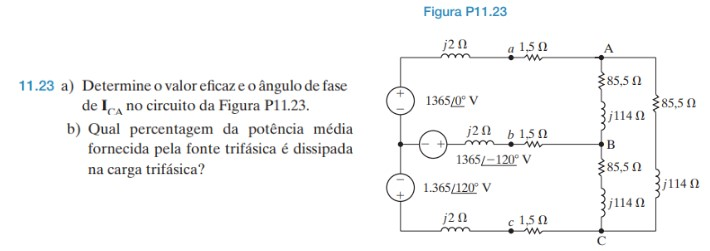
\includegraphics[scale=1.0]{P11.23.jpg}
\end{center}

\subsection*{(a)}

Como o circuito trifásico do enunciado é equilibrado, o primeiro passo é encontrar o circuito monofásico equivalente. \\
Para isso, aplicamos conversão delta - estrela na carga trifásica conectada à fonte. Quando todas impedâncias são iguais,
temos que a conversão de uma impedância em $\Delta$ para $Y$ é feita via

\begin{equation}\label{eq:11.23.1}
    Z_{Y} = \frac{Z_{\Delta}}{3}
\end{equation}

Assim, temos que configuração $Y$ da carga do problema possui impedância de fase dada por   

\[ Z_Y = \frac{85.5 + j114}{3} = 28.5 +j38 \un{$\Omega$} \]

Assim, o circuito monofásico equivalente da fase $a$ está exibido na Figura \ref*{fig:11.23.1}

Combinando as impedâncias de fase e carga, e usando o fato que a fonte da fase $c$ está desconectada do neutro da fonte trifásica, 
temos o circuito equivalente mostrado na Figura \ref*{fig:11.23.1}.

\begin{figure}[hb]
    \centering
    \caption{Circuito monofásico equivalente da fase $a$.}
      \centering
      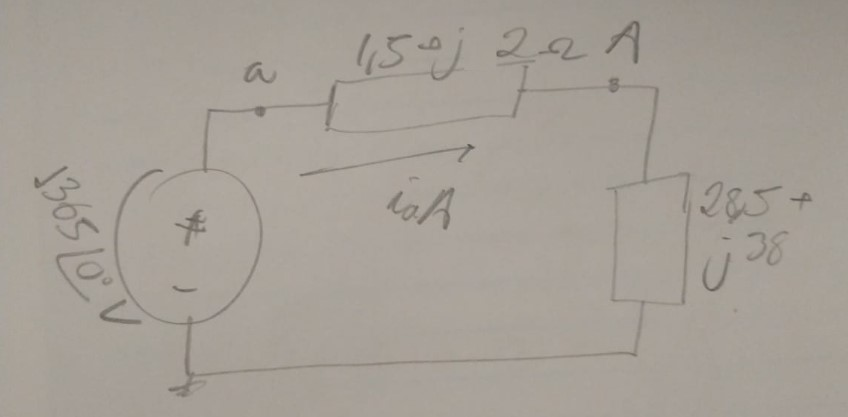
\includegraphics[scale=0.5]{P11.23-Item(a).jpg} \\
    \label{fig:11.23.1}
\end{figure}

Nesse circuito equivalente, temos que a corrente de fase $I_{aA}$ é   

\[ I_{aA} = \frac{1365}{30 + j40} = 27.31\phase{-53.13^{\circ}} \un{A} \]

Assim, como as correntes de dase em um circuito equilibrado tem módulo igual mas defesagem de $120^{\circ}$, temos  

\[ I_{bB} = 27.31\phase{-173.13^{\circ}} \un{A} \quad , \quad I_{cC} = 27.31\phase{66.87^{\circ}} \un{A} \]

Note que as tensões de fase são positivas (ordem $abc$), logo as correntes também possuem essa ordem.
Usando $I_{cC}$, temos que a queda de tensão $V_{cn}$ em cada fase da carga na configuração $Y$ é  

\[ V_{cn} = I_{cC} \cdot Z_Y \]

\[ V_{cn} = 27.31\phase{66.87^{\circ}} \cdot (28.5 +j38 ) = 1296.78\phase{120^{\circ}} \un{V} \]

Uma vez conhecido a tensão de fase $V_{cn}$ na carga, temos que a tensão de linha $V_{CA}$ na carga é

\begin{equation}\label{eq:11.23.2}
    V_{CA} = \sqrt{3}|V_{cn}|\phase{\phi_{cn} + 30^{\circ}}
\end{equation}

Substituindo, temos    

\[ V_{CA} = 2246\phase{150^{\circ}} \un{V} \]

Finalmente, a corrente de linha $I_{CA}$ na configuração $\Delta$ é  

\[ I_{CA} = \frac{V_{CA}}{Z_{\Delta}} = \frac{2246\phase{150^{\circ}}}{85.5 + j114} \]

\[ \boxed{I_{CA} = 15.46\phase{96.86^{\circ}} \un{A}} \]

\subsection*{(b)}

Usando o circuito monofásico equivalente da Figura \ref*{fig:11.23.1}, temos que a potência fornecida pela fonte por fase é  

\[ S_{V/\phi} = V_{An} \cdot (I_{aA})^* = 37278.15\phase{53.13^{\circ}} \un{VA} \]

A potência que efetivamente chega na carga por fase é 

\[ S_{L/\phi} = V_{an} \cdot (I_{aA})^* \]

Podemos usar a fase $c$ que já conhecemos o valor de $V_{cn}$, usando o fato do circuito equilibrado dissipar a mesma
potência em todas as fases.

\[ S_{L/\phi} = V_{cn} \cdot (I_{cC})^* = 31415.06\phase{53.13^{\circ}} \un{VA} \]

A porcentagem $S_{\%}$ da potência fornecida pela fonte que chega na carga é  

\[ S_{\%} = \frac{S_{L/\phi}}{S_{V/\phi}} = \frac{31415.06\phase{53.13^{\circ}} \un{VA}}{37278.15\phase{53.13^{\circ}} \un{VA}} \, 100\% \]

\[ \boxed{S_{\%} = 84.27\%} \]

